\chapter{Design Front-End}

%capo la mia conoscenza di latex si sta espandendo però probabilmente questo non compila comunque, halp me plz
% ho fatto del mio meglio per preparare un brodo degno di gordon ramsay
% by @Boss314

\section{Pagina Iniziale}

    \label{fig:4.1}
    \begin{figure}[H]
        \center
        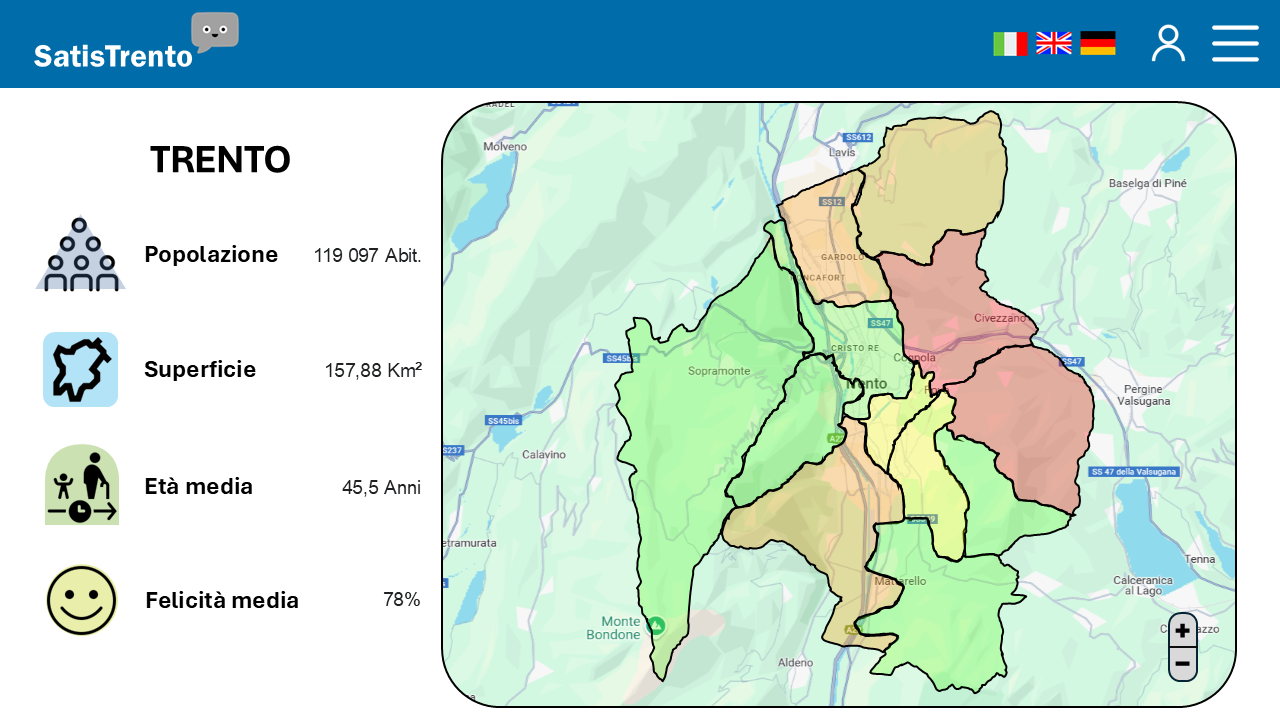
\includegraphics[width=0.6\textwidth]{Interfaccia_grafica/home.PNG}
        \caption{Schermata principale dell'applicazione}
    \end{figure}

    La Figura 4.1 mostra un mockup della pagina principale dell'applicazione, questa schermata sarà visibile a tutti gli utenti, loggati e non loggati.

    \begin{itemize}
        \item \textbf{RF1: Homepage} \begin{itemize}
            \item La homepage dell'applicazione mostra la mappa del Comune di Trento in primo piano, sono visibili anche i confini tra i singoli quartieri della città.
        \end{itemize}
        \item \textbf{RF3: Multi lingua} \begin{itemize} 
                \item L'interfaccia contiene tre pulsanti, ognuno contenente una bandiera corrispondente a una delle lingue supportate dall'applicazione (italiano, inglese, tedesco). Cliccando sui pulsanti cambierà la lingua in cui è presentata l'applicazione.
        \end{itemize}
        \item \textbf{RF6: Autenticazione} \begin{itemize} 
            \item L'interfaccia presenta un pulsante, rappresentato da un'icona a forma di "persona", che permette di iniziare il processo di autenticazione degli utenti. Questo permette agli utenti loggati di acceder al proprio account tramite SPID, CNS, CIE, CPS; come dettato dal requisito.
        \end{itemize}
        \item \textbf{RNF10: Facilità d’uso} \begin{itemize}
                \item La grafica disponibile a tutti gli utenti utilizza un design chiaro, usando icone per rendere la navigazione dell'interfaccia il più accessibile e intuitiva possibile. 
        \end{itemize}
        \item \textbf{RNF11: Facilità di navigazione} \begin{itemize}
            \item L'interfaccia permette all'utente di navigare facilmente tra le pagine, inoltre è possibile accedere a tutte le funzionalità dell'applicazione (se l'utente risulterà loggato) tramite il menù a tendina, che si apre cliccando sull'icona ad "hamburger" presente nella parte superiore destra della schermata.
        \end{itemize}
        \item \textbf{RNF12: Multilingua} \begin{itemize} 
            \item All'inizio, l'interfaccia sarà presentata in lingua italiana. Il design include pulsanti, sempre presenti nella parte alta della schermata, per cambiare la lingua in inglese o tedesco.
        \end{itemize}
    \end{itemize}


\newpage
\section{Utente Loggato, Dati in Tabella}

    \begin{figure}[H]
        \center
        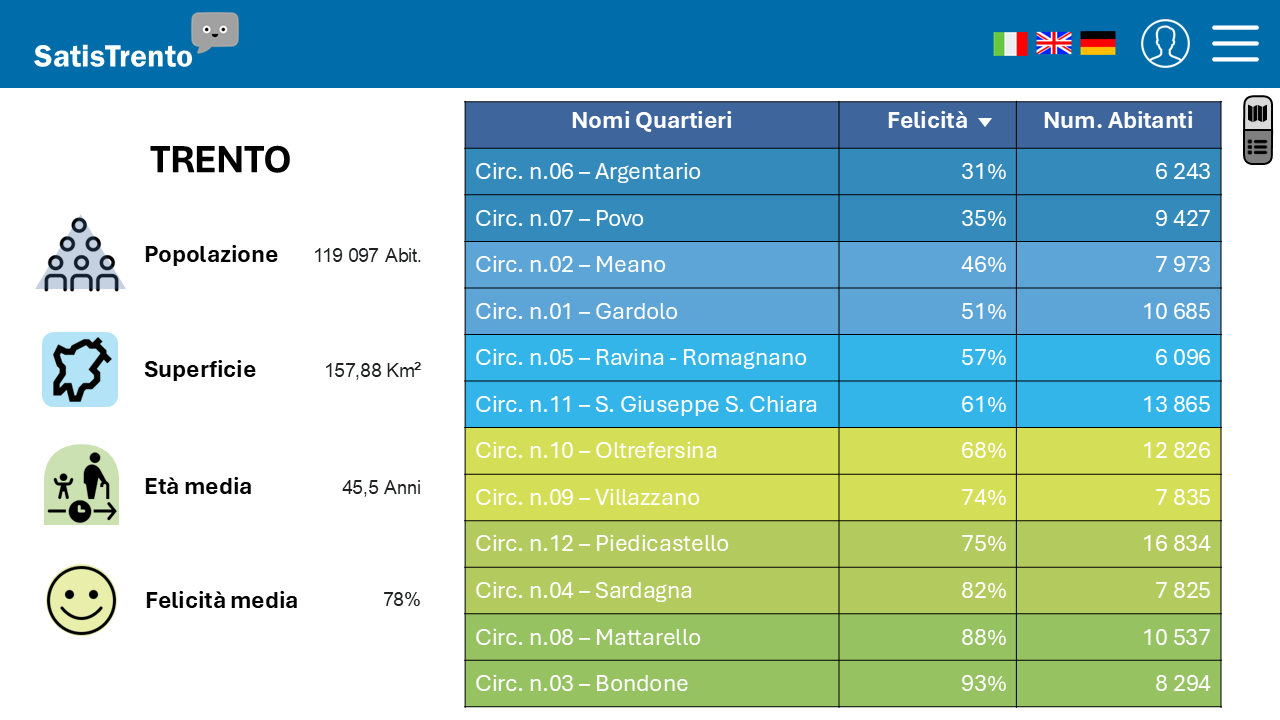
\includegraphics[width=0.6\textwidth]{Interfaccia_grafica/dataDetail.PNG}
        \caption{Dettaglio dati per analisti e amministratori}
    \end{figure}    

    La Figura 4.2 mostra il mockup della schermata di homepage modificata visibile agli utenti di tipo: analista, circoscrizione e amministratore. Questa schermata sarà visibile solo dopo che l'utente ha effettuato l'accesso e sarà visibile solo agli utenti con i privilegi sopra citati.

    \begin{itemize}
        \item \textbf{RF6: Autenticazione} \begin{itemize} 
            \item Inoltre è presente il pulsante per aprire il menù a tendina per permettere all'utente di usufruire delle funzionalità abilitate al proprio account e di eseguire il logout.
        \end{itemize}
        \item \textbf{RF7: Cambio icona login} \begin{itemize} 
            \item L'icona di login è sostituita da un'icona differente per simboleggiare l'accesso eseguito. Questo permette all'utente di individuare l'account con il quale si ha fatto il login
        \end{itemize}
        \item \textbf{RF12: Modifica Homepage} \begin{itemize}
            \item Sebbene il mockup mostri i dati dell'applicazione in una tabella, questa funzionalità sarà disponibile solo quando l'utente è loggato come analista, amministratore o circoscrizione. Tutti gli utenti loggati senza privilegi speciali vedranno solo i dati generali, come mostrato nella \hyperref[fig:4.1]{Figura 4.1}.
            \item Inoltre se si preferisce la visualizzazione tramite "mappa" sarà possibile passare a questa tramite icone presenti nella parte destra della mappa sull'angolo in alto. 
        \end{itemize}
        \item \textbf{RF13: Accesso come analista, circoscrizione o amministratore} \begin{itemize}
            \item Gli utenti: analisti, circoscrizioni e amministratori, dopo aver eseguito l'accesso verranno reindirizzati alla presente interfaccia.
        \end{itemize}
        \item \textbf{RNF10: Facilità d’uso} \begin{itemize}
            \item L'interfaccia è stata progettata per essere il più intuitiva possibile, i dati sono presentati in una tabella la quale potrà essere ordinata e filtrata per facilitare la consultazione. Il tutto tramite pulsanti e icone facilmente riconoscibili. Quali le icone di "mappa" e "tabella" per cambiare la visualizzazione dei dati, oppure le icone di "freccia" per ordinare i dati in base a una colonna specifica.
        \end{itemize}
        \item \textbf{RNF11: Facilità di navigazione} \begin{itemize}
            \item L'interfaccia permette all'utente di navigare facilmente tra le pagine, inoltre è possibile accedere a tutte le funzionalità dell'applicazione tramite il menù a tendina, che si apre cliccando sull'icona standard ad "hamburger" presente nella parte superiore destra della schermata.
            \end{itemize}
    \end{itemize}
\newpage
\section{Selezione di un Quartiere}
    \begin{figure}[H]
        \center
        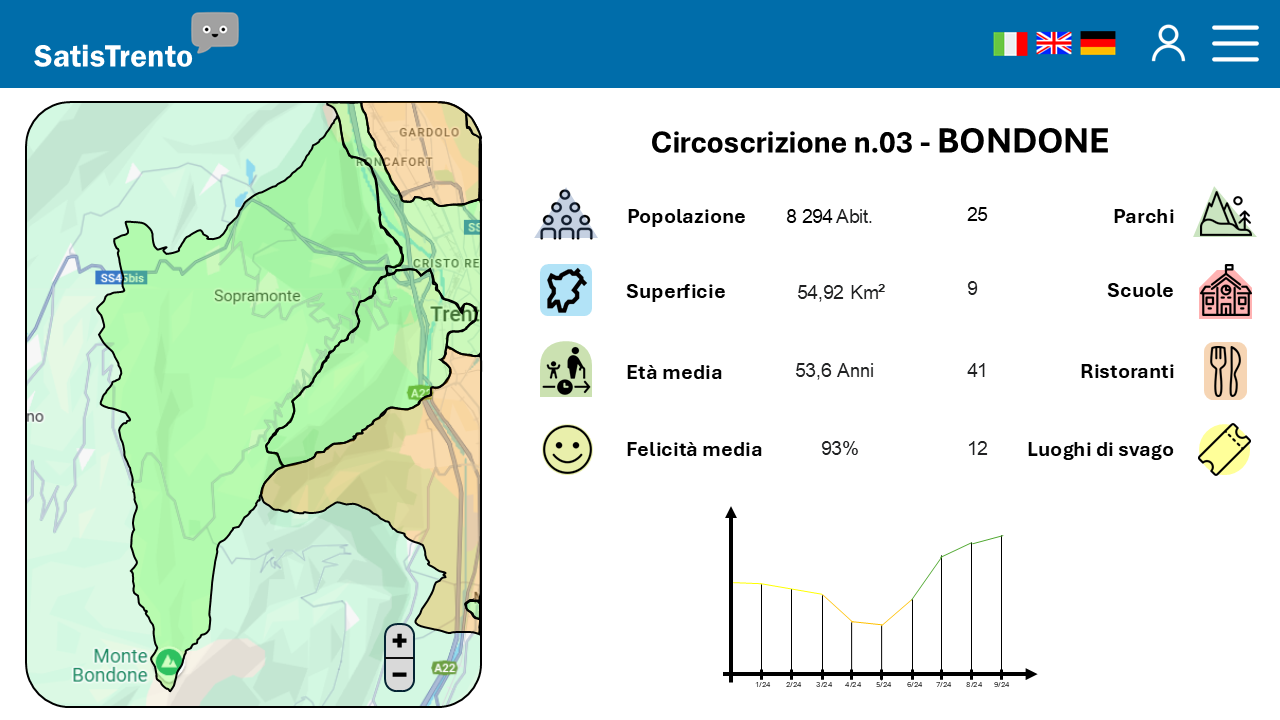
\includegraphics[width=0.6\textwidth]{Interfaccia_grafica/quartiereSelected.PNG}
        \caption{Dettaglio dati per un quartiere selezionato}
    \end{figure}    

    La Figura 4.3 mostra il mockup della schermata visibile dopo che l'utente ha cliccato su uno dei quartieri presenti nella mappa.

    \begin{itemize}
        \item \textbf{RF4: Accesso dati quartieri} \begin{itemize}
            \item Selezionare un quartiere è possibile cliccandolo sulla mappa. Una volta che un quartiere è selezionato la mappa lo mostra al centro e ingrandito, e le informazioni relative a esso vengono presentate al fianco della mappa. Nel mockup l'interfaccia mostra solo i dati generali, visibili dagli utenti non loggati. Ma agli account abilitati è consentito osservare anche i dati più approfonditi.
        \end{itemize} 
        \item \textbf{RF15: Visualizzazione Analisi Storico} \begin{itemize}
            \item Si noti che è presente un grafico che mostra l'\textbf{andamento nel tempo} del grado di soddisfazione del quartiere selezionato. 
            \item Nonostante il grafico, e l'analisi nel tempo, sia un requisito specifico per utenti analisti, si è deciso di includere suddetto requisito in quanto questo è un esempio di come l'interfaccia può risultare lato analista.
        \end{itemize}
    \end{itemize}
\section{Caricamento sondaggi e modifica dati}
    \label{fig:4.4}
    \begin{figure}[H]
        \center
        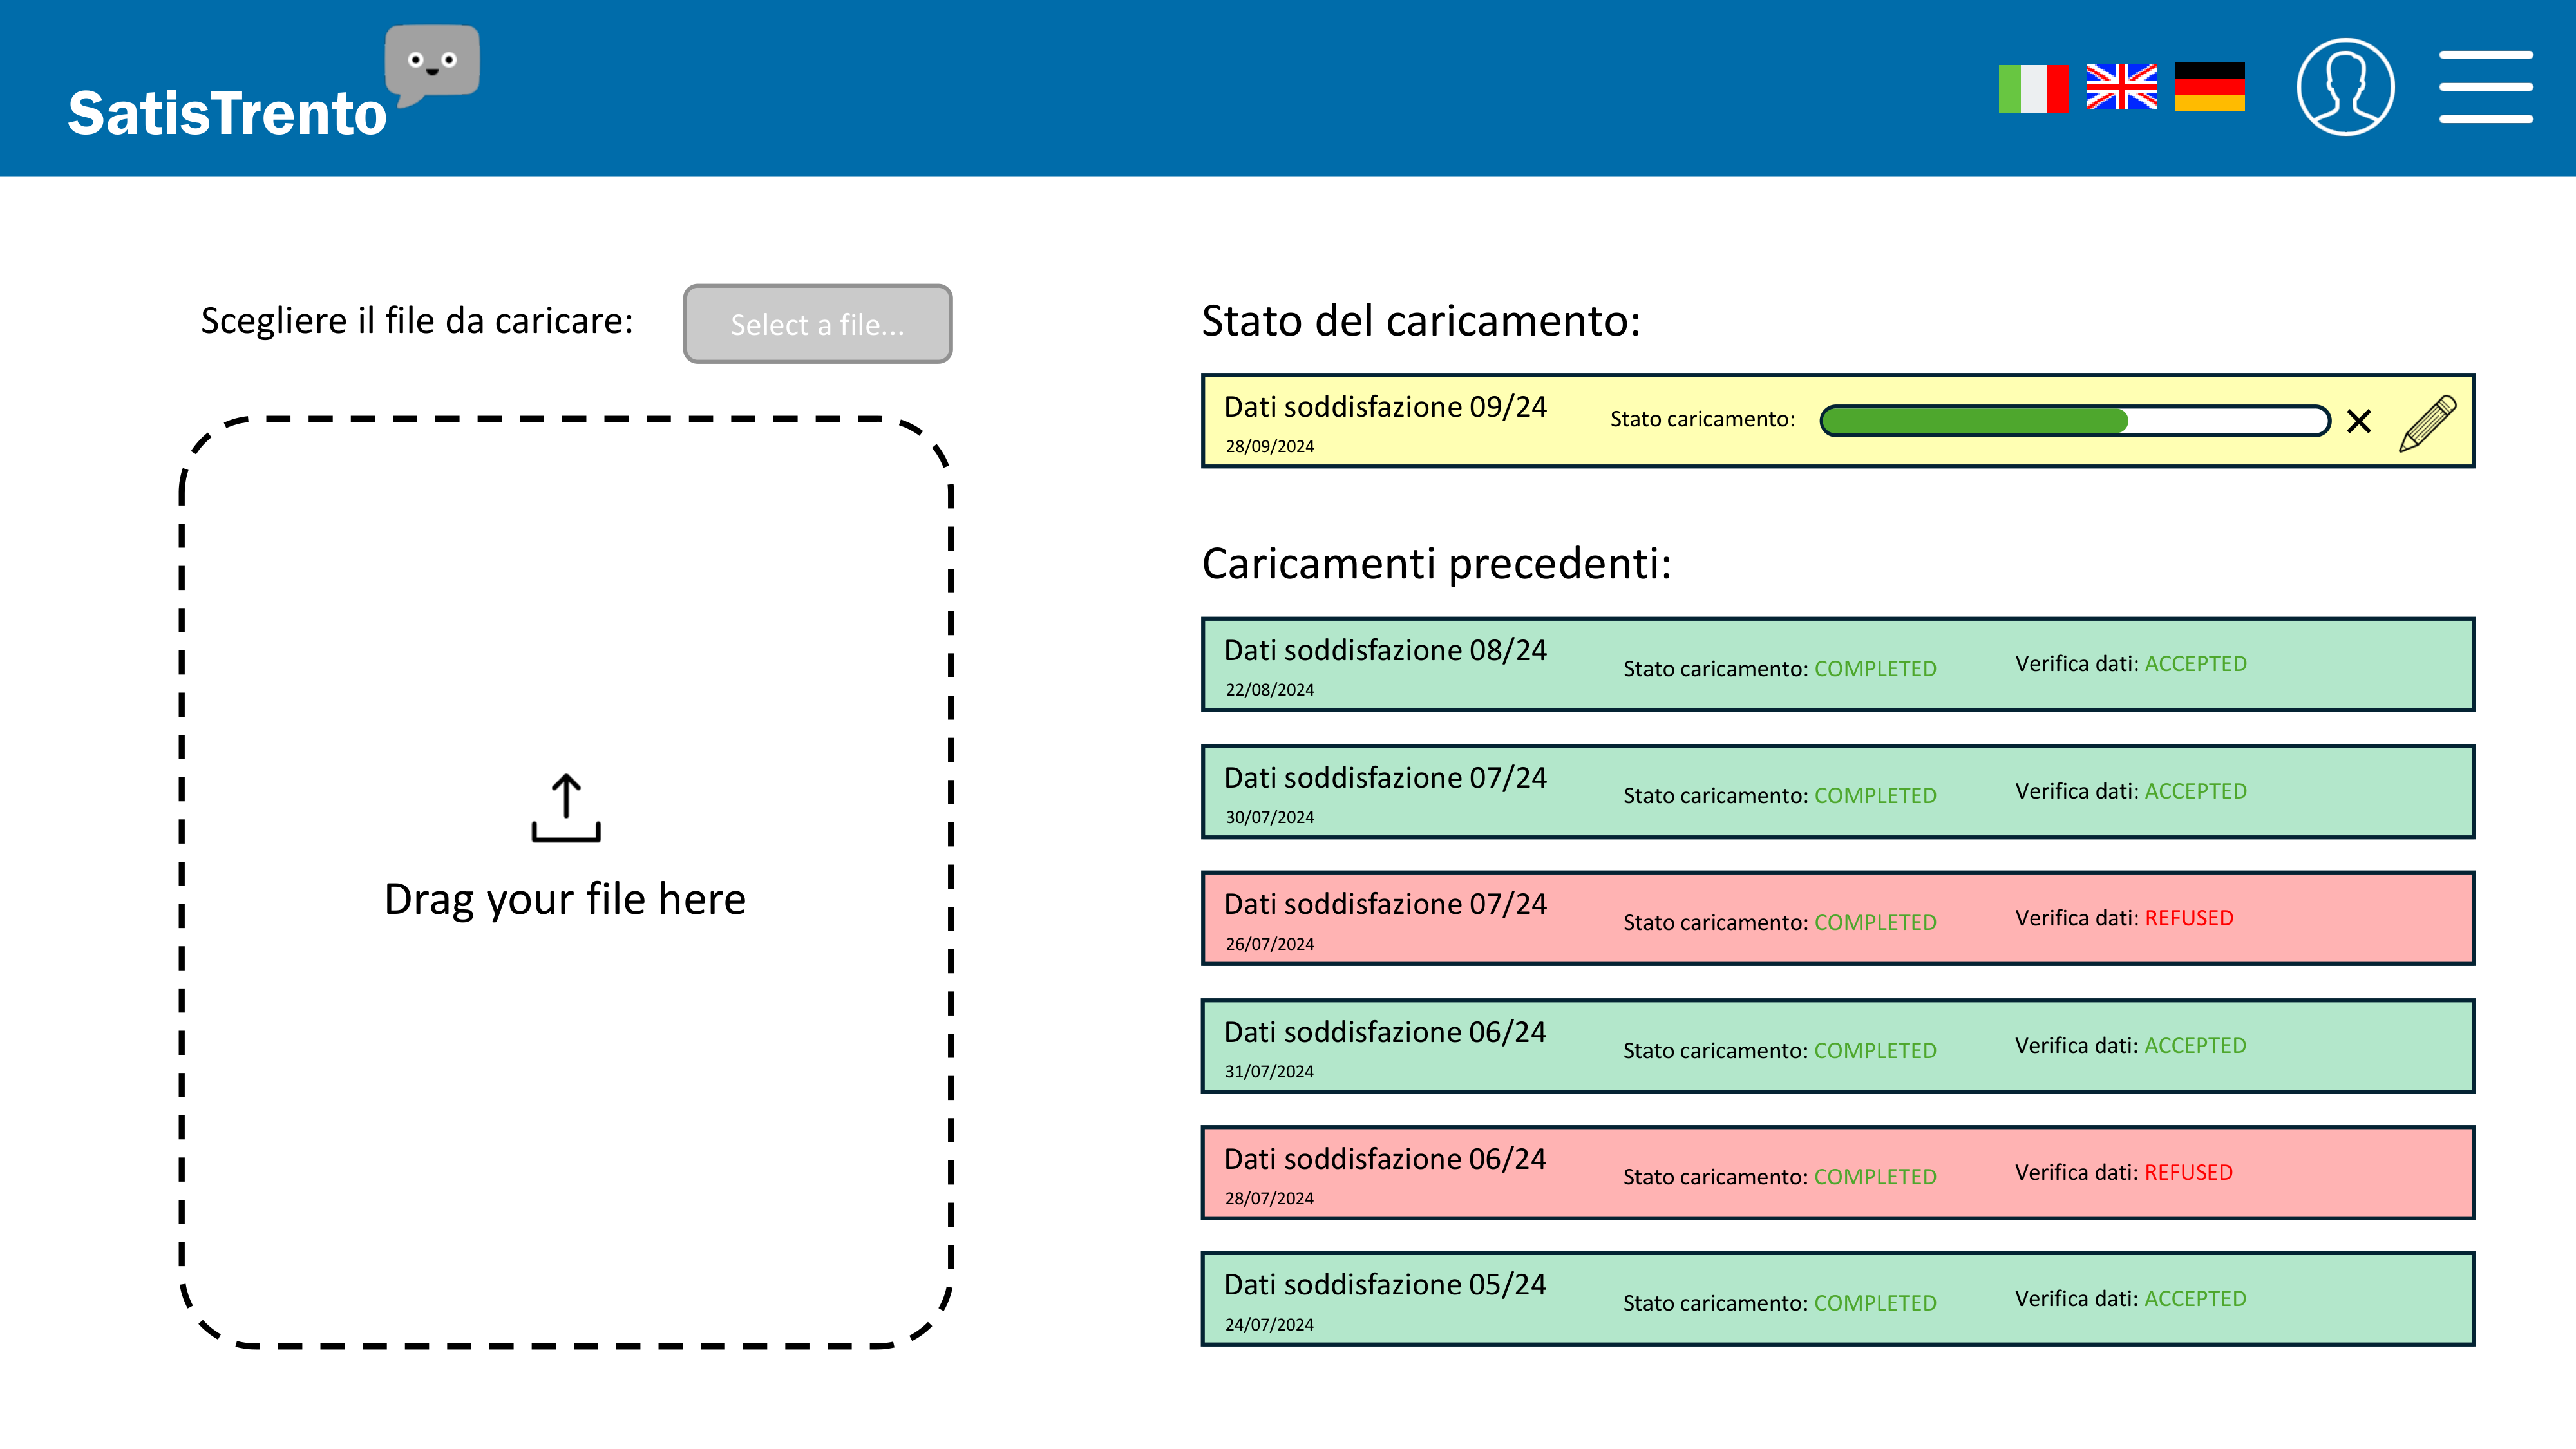
\includegraphics[width=0.6\textwidth]{Interfaccia_grafica/uploadData.PNG}
        \caption{Caricamento dati e visualizzazione elenco}
    \end{figure} 
    La figura 4.4 mostra il mockup della schermata visibile ai sondaggisti e agli amministratori, in cui è possibile caricare i dati sui sondaggi effettuati.\newline
    Il presente layout sarà la base le visualizzazioni lato amministratore per la gestione dei dati e utenti.
    \begin{itemize}
        \item \textbf{RF8: Visualizzazione dati sondaggisti} \begin{itemize}
            \item La seguente pagina permetterà ai sondaggisti di visualizzare i dati caricati da loro stessi, inoltre è presente per ogni sondaggio lo stato di approvazione da parte degli amministratori.
        \end{itemize}
        \item \textbf{RF9: Accesso come sondaggista} \begin{itemize}
            \item Gli utenti: sondaggisti, dopo aver effettuato l'accesso verranno reindirizzati alla presente interfaccia la quale sarà inoltre disponibile solamente a tale tipologia di utente
        \end{itemize}
        \item \textbf{RF10: Creazione nuovi sondaggi} \begin{itemize}
            \item La presente interfaccia permette agli utenti di tipo sondaggista caricare un file contenente un sondaggio effettuato in precedenza. Inoltre permette di creare un nuovo sondaggio, inserendo i dati generali.
            \item La seguente pagina fungerà da accesso per la modifica e/o eliminazione di dati caricati da sondaggisti non ancora approvati.
        \end{itemize}
        \item \textbf{RF16-17-18-20: Approvazione e disapprovazione sondaggi, modifica dati statici, modifica utenti abilitati} \begin{itemize}
            \item Sebbene la figura rappresenti l'interfaccia delle funzioni per gli utenti sondaggisti, un layout simile può essere usato per l'interfaccia degli utenti amministratori. Tabelle, come quella visibile nella figura, possono essere usate per mostrare i dati statici memorizzati nel sistema e i sondaggi inseriti dai sondaggisti per approvarli o rifiutarli. Un'altra interfaccia simile può permettere agli amministratori di visualizzare e modificare la lista degli utenti loggati e dei loro privilegi.
        \end{itemize} 
        \item \textbf{RNF6: Capacità di caricamento} \begin{itemize}
            \item Questa sarà la principale pagina di caricamento dati sull'applicazione una volta che sull'applicazione saranno caricati i dati di base. In quanto i dati dei sondaggi potrebbero essere pesanti e numerosi, l'interfaccia dovrà essere in grado di gestire il caricamento di grandi quantità di dati in breve tempo.
        \end{itemize}
        \item \textbf{RNF10: Facilità d’uso} \begin{itemize}
            \item Si nota come l'interfaccia è intuitiva e permette all'utente di capire facilmente come caricare i dati e come vedere l'elenco delle informazioni già caricate.
        \end{itemize}
    \end{itemize}




\section{Creazione nuovo sondaggio}

    \begin{figure}[H]
        \center
        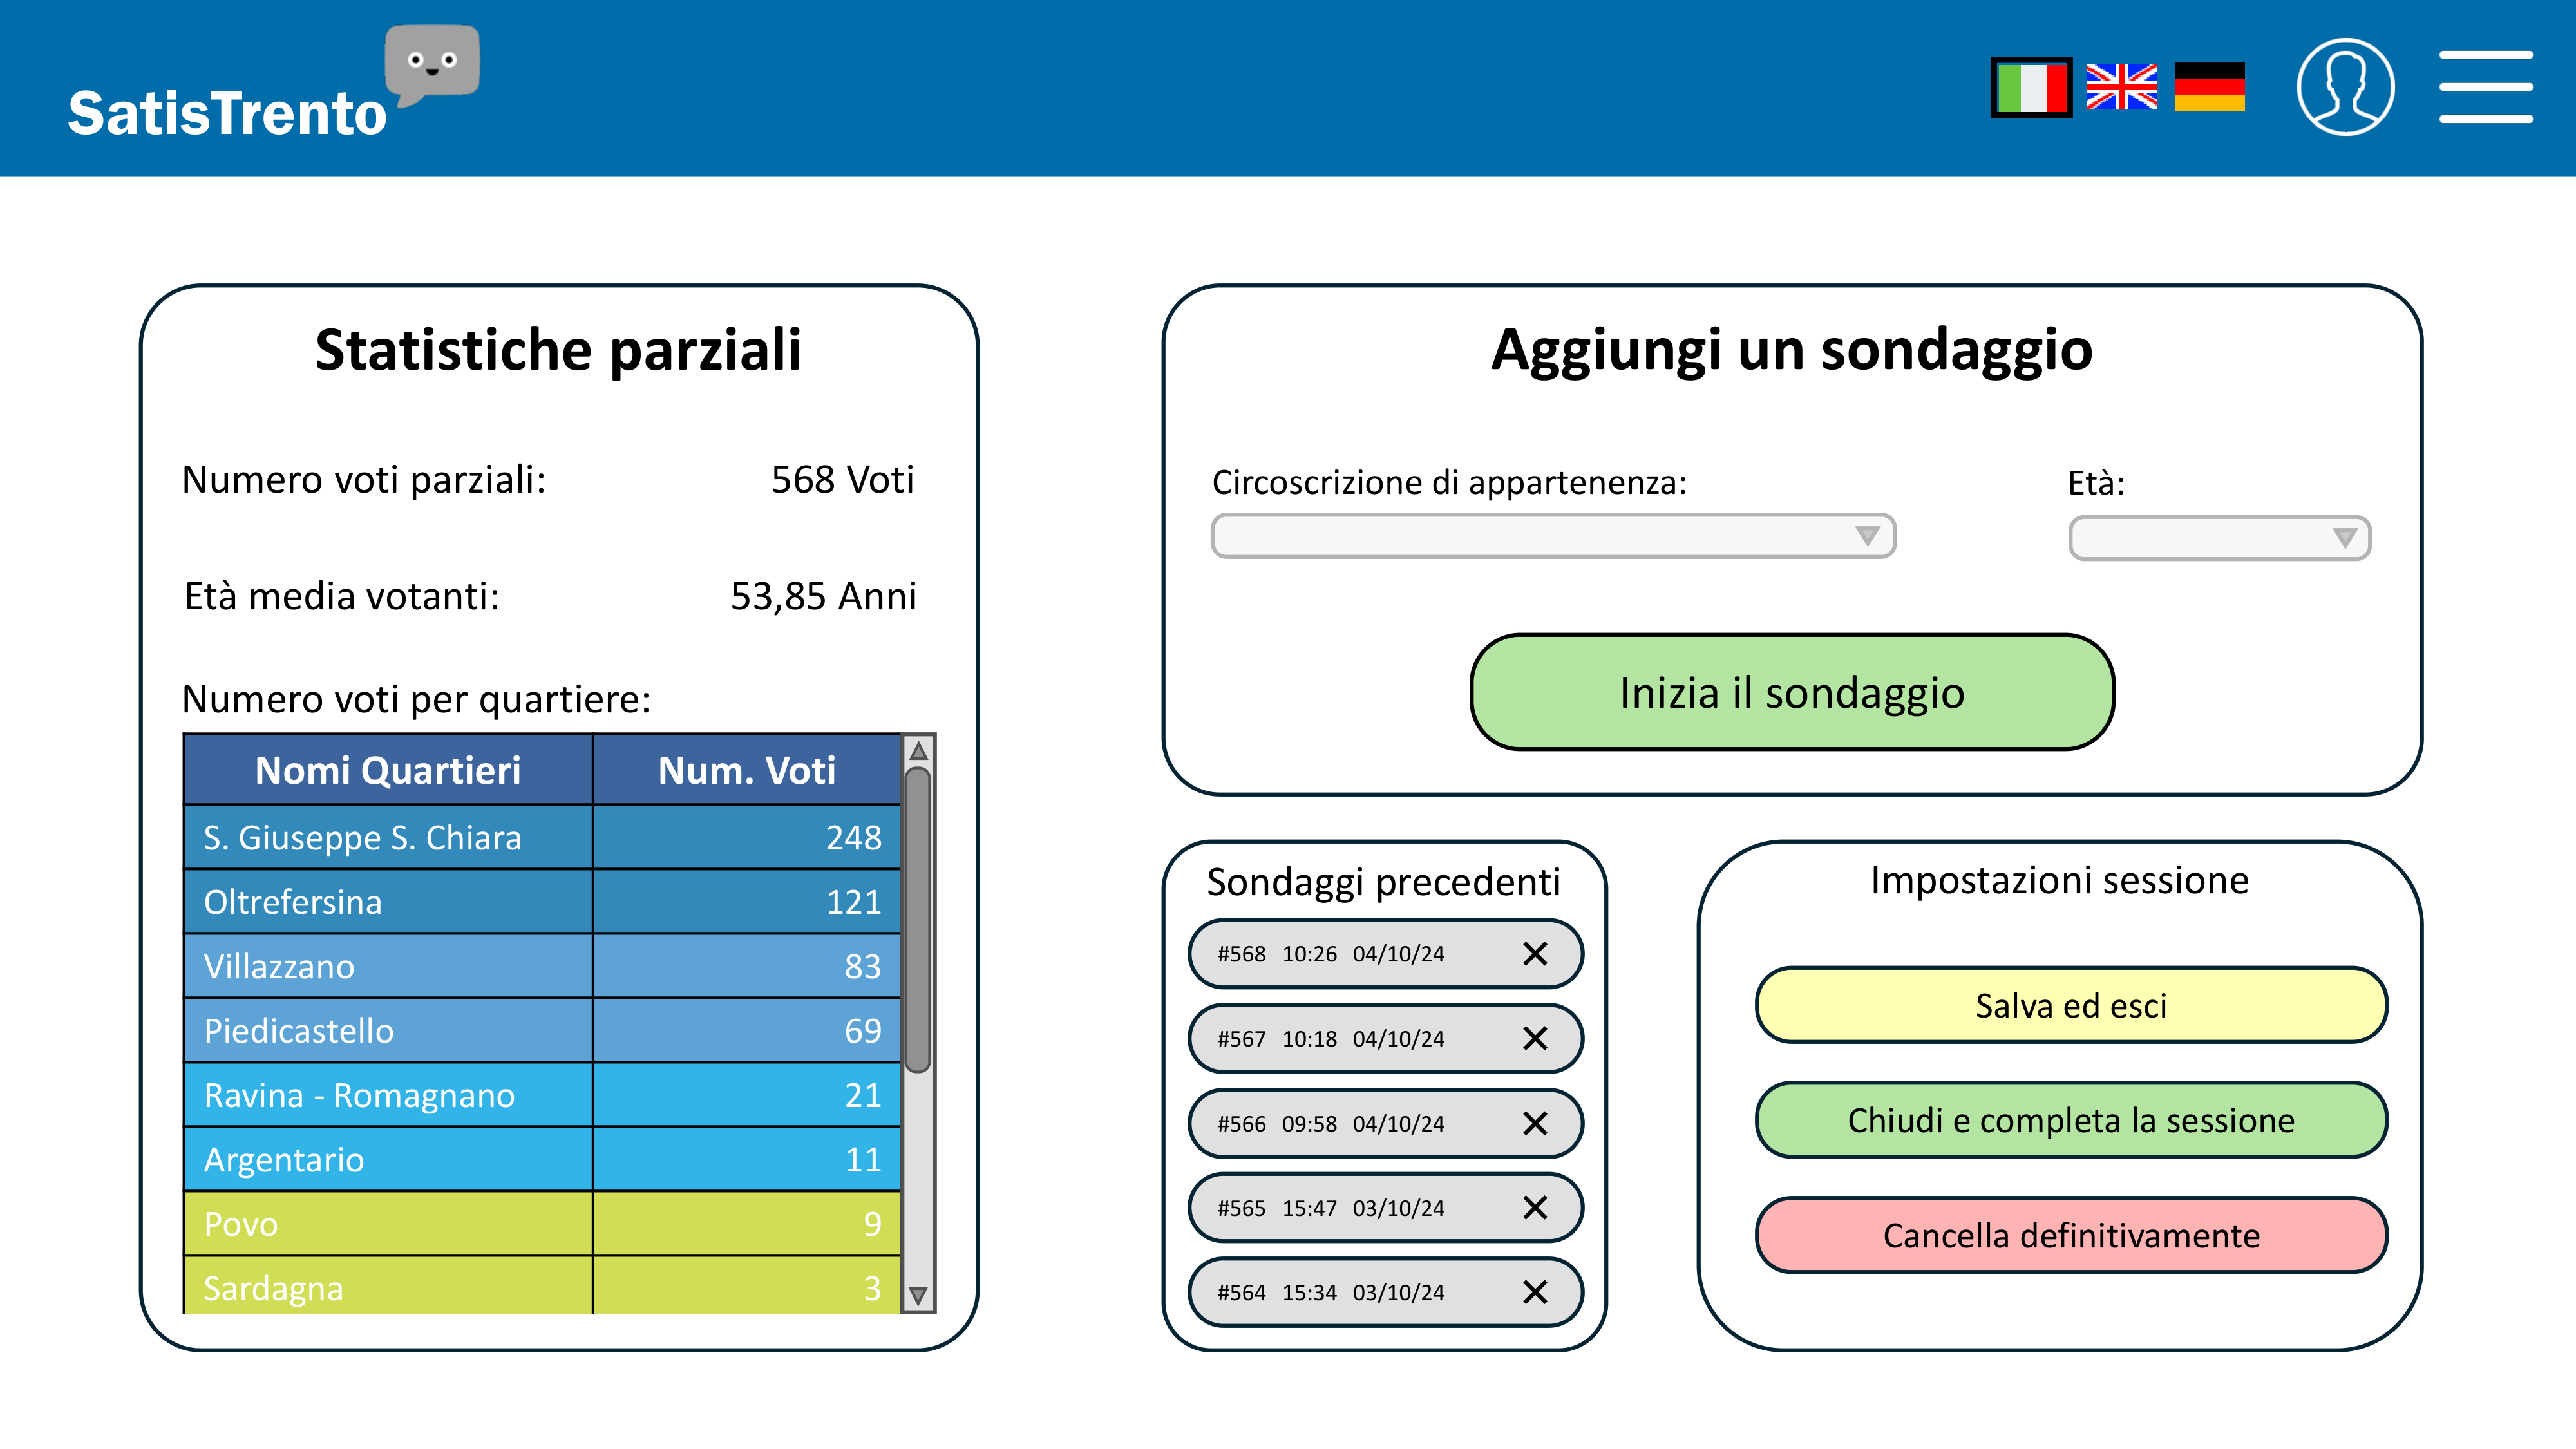
\includegraphics[width=0.6\textwidth]{Interfaccia_grafica/newSurvey.PNG}
        \caption{Schermata della sessione di sondaggio}
    \end{figure}

    La figura 4.5 mostra il mockup della schermata visibile ai sondaggisti durante una sessione di sondaggio. L'interfaccia mostra informazioni sul sondaggio attuale.

    \begin{itemize}
        \item \textbf{RF11: Svolgimento sondaggi} \begin{itemize}
            \item L'interfaccia permette ai sondaggisti di aggiungere nuovi voti al sondaggio attuale, selezionando circoscrizione di appartenenza e età.
            \item Da questa interfaccia è anche possibile: visualizzare i dati raccolti fino a quel momento, chiudere la sessione di sondaggio e inviare i dati per la revisione, sospendere la sessione per continuare in un secondo momento oppure eliminare tutti i dati raccolti fino a quel momento.
            \item Infine sempre dalla seguente interfaccia è possibile vedere un elenco dei voti raccolti fino a quel momento, con la possibilità di eliminare i voti singolarmente.
        \end{itemize}
    \end{itemize}
    